% Chapter 2



\chapter{Literature Study} % Main chapter title

\label{Literature Study} % For referencing the chapter elsewhere, use \ref{Chapter1} 

%----------------------------------------------------------------------------------------

% Define some commands to keep the formatting separated from the content 

%----------------------------------------------------------------------------------------

\section{Knowledge Discovery Steps}
Knowledge Discovery is the non-trivial process of identifying valid, novel, potentially useful, and ultimately understandable patterns in data \\\cite{knowledge discovery}. With the emphasis on collecting data increasing around the world, there is an urgent need for a new generation of different techniques, methods and algorithms to assist researchers, analysts, decision makers and managers in extracting useful patterns from the rapidly growing volumes of data. These techniques and tools are the subject of the emerging field of knowledge discovery in databases .Knowledge Discovery and Data Mining  is an interdisciplinary area focusing upon methodologies for extracting useful knowledge from data.Knowledge Discovery and Data Mining is an interdisciplinary area focusing upon methodologies for extracting useful knowledge from data.According to \cite{IBM}, Though Knowledge Discovery is used synonymously to represent data mining, both these are actually different. Some preprocessing steps before data mining and post processing steps after data mining are to be completed to transform the raw data as useful knowledge. \newline
Knowledge Discovery is an iterative process that transforms raw data into useful information. Different steps of Knowledge Discovery in Databases are discussed in \cite{kddsteps}.

\begin{figure}
\centering
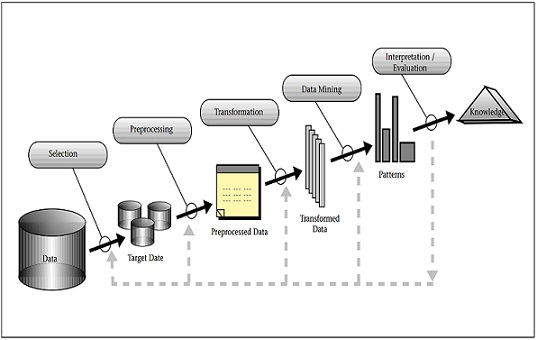
\includegraphics{Figures/kdsteps.jpg}
\decoRule
\caption{Knowledge discovery steps}
\label{fig:kdsteps}
\end{figure}



Figure \ref{fig:kdsteps} shows the general process of knowledge discovery.

\subsection{Understanding the Application Domain}
The first step is understanding requirements.It is needed to have a clear understanding about the application domain and your objectives.It should be also known whether the data is going to be described or information is predicted.
\subsection{Selection of Dataset}
Data mining is done on current or past records. Thus,a data set or subset of data should be selected, in other words data samples, on which you need to perform data analysis and get useful knowledge.There should be enough quantity of data to perform data mining.
\subsection{Data Cleaning}
Data cleaning is the step where noise and irrelevant data are removed from the large data set. This is a very important preprocessing step because the outcome would be dependent on the quality of selected data. As part of data cleaning, duplicate records might have to be removed, logically correct values for missing records might have to be entered, unnecessary data fields might have to be removed, data format standardized, update data in a timely manner and so on.
\subsection{Data transformation}
With the help of dimensionality reduction or transformation methods, the number of effective variables is reduced and only useful features are selected to depict data more efficiently based on the goal of the task. In short, data is transformed into appropriate form making it ready for data mining step.
\subsection{Finding interesting features in the database}
This step is extremely important in the field of International Studies. Researchers and practitioners with different backgrounds and different languages may work on a given database, getting different results. Each group may consider different attributes in doing so.
\subsection{Selection of data mining task}
Based on the objective of data mining, appropriate task is selected. Some common data mining tasks are classification, clustering, association rule discovery, sequential pattern discovery, regression and deviation detection. You can choose any of these tasks based on whether you need to predict information or describe information.
\subsection{Selection of Data mining method}
Appropriate method(s) is to be selected for looking for patterns from the data. You need to decide the model and parameters that might be appropriate for the method. Some popular data mining methods are decision trees and rules, relational learning models, example based methods etc.
\subsection{Data mining}
Data mining is the actual search for patterns from the data available using the selected data mining method.
\subsection{Pattern evaluation}
This is a post processing step in KDD which interprets mined patterns and relationships. If the pattern evaluated is not useful, then the process might again start from any of the previous steps, thus making KDD an iterative process.
\subsection{Knowledge consolidation}
This is the final step in Knowledge Discovery. The knowledge discovered is consolidated and represented to the user in a simple and easy to understand format. Mostly, visualization techniques are being used to make users understand and interpret information. \newline

Though these are the main steps in any Knowledge Discovery process, some of the steps could be done combined during the actual process.  For example, considering the convenience, data selection and data transformation can be combined together. Even after presenting knowledge to the user, new data can be added to the data set or mining can be further refined or a different data mining method can be chosen to get more accurate results. Thus, Knowledge Discovery is completely an iterative process.


%----------------------------------------------------------------------------------------

\section{Data Mining Concepts}

\paragraph{}
Data mining is the process of discovering interesting patterns and knowledge from large amounts of data. The
data sources can include databases, data warehouses, the Web, other information repositories, or data that are
streamed into the system dynamically.
\begin{figure}
   \centering
  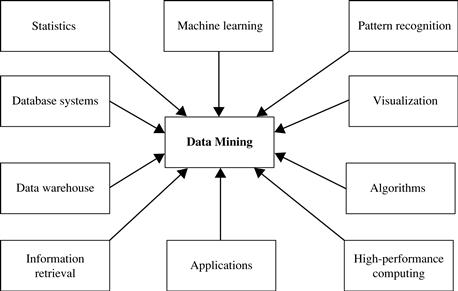
\includegraphics[width=\linewidth]{Figures/datamining.jpg}
  \decoRule
  \caption[Data Mining]{Data Mining Concept}
  \label{fig:datamining}
\end{figure}

Figure \ref{fig:datamining} shows the general parts of data mining.
As a general technology, data mining can be applied to any kind of data as long as the data are meaningful for a
target application. The most basic forms of data for mining applications are database data, data warehouse data, and transactional data.
\subsection{Database Data}
\paragraph{}
A database system, also called a database management system (DBMS), consists of a collection of
interrelated data, known as a database, and a set of software programs to manage and access the data. The
software programs provide mechanisms for defining database structures and data storage; for specifying and
managing concurrent, shared, or distributed data access; and for ensuring consistency and security of the
information stored despite system crashes or attempts at unauthorized access.
\paragraph{}
A relational database is a collection of tables, each of which is assigned a unique name. Each table consists of
a set of attributes (columns or fields) and usually stores a large set of tuples (records or rows). Each tuple in a
relational table represents an object identified by a unique key and described by a set of attribute values. A
semantic data model, such as an entity-relationship (ER) data model, is often constructed for relational
databases. An ER data model represents the database as a set of entities and their relationships.

\subsection{Data Warehouses}
\paragraph{}
A data warehouse is usually modeled by a multidimensional data structure, called a data cube, in which each
dimension corresponds to an attribute or a set of attributes in the schema, and each cell stores the value of
some aggregate measure such as count or sum. A data cube provides a multidimensional view of
data and allows the precomputation and fast access of summarized data.

\subsection{Transactional Data}
\paragraph{}
In general, each record in a transactional database captures a transaction, such as a customer\'s purchase, a
flight booking, or a user's clicks on a web page. A transaction typically includes a unique transaction identity
number (trans\_ID) and a list of the items making up the transaction, such as the items purchased in the
transaction. A transactional database may have additional tables, which contain other information related to the
transactions, such as item description, information about the salesperson or the branch, and so on.


\subsection{Other Kinds of Data}
\paragraph{}
Besides relational database data, data warehouse data, and transaction data, there are many other kinds of data
that have versatile forms and structures and rather different semantic meanings. Such kinds of data can be seen
in many applications: time-related or sequence data (e.g., historical records, stock exchange data, and timeseries and biological sequence data), data streams (e.g., video surveillance and sensor data, which are
continuously transmitted), spatial data (e.g., maps), engineering design data (e.g., the design of buildings,
system components, or integrated circuits), hypertext and multimedia data (including text, image, video, and
audio data), graph and networked data (e.g., social and information networks), and the Web (a huge, widely
distributed information repository made available by the Internet). These applications bring about new
challenges, like how to handle data carrying special structures (e.g., sequences, trees, graphs, and networks)
and specific semantics (such as ordering, image, audio and video contents, and connectivity), and how to mine
patterns that carry rich structures and semantics.
\\
Various kinds of knowledge can be mined from these kinds of data. Here, we list just a few. Regarding
temporal data, for instance, we can mine banking data for changing trends, which may aid in the scheduling of
bank tellers according to the volume of customer traffic. Stock exchange data can be mined to uncover trends
that could help you plan investment strategies. \\We could
mine computer network data streams to detect intrusions based on the anomaly of message flows, which may
be discovered by clustering, dynamic construction of stream models or by comparing the current frequent
patterns with those at a previous time. With spatial data, we may look for patterns that describe changes in
metropolitan poverty rates based on city distances from major highways. The relationships among a set of
spatial objects can be examined in order to discover which subsets of objects are spatially autocorrelated or
associated. By mining text data, such as literature on data mining from the past ten years, we can identify the
evolution of hot topics in the field. By mining user comments on products (which are often submitted as short
text messages), we can assess customer sentiments and understand how well a product is embraced by a
market. From multimedia data, we can mine images to identify objects and classify them by assigning semantic
labels or tags. By mining video data of a hockey game, we can detect video sequences corresponding to goals.
Web mining can help us learn about the distribution of information on the WWW in general, characterize and
classify web pages, and uncover web dynamics and the association and other relationships among different web
pages, users, communities, and web-based activities.\\
It is important to keep in mind that, in many applications, multiple types of data are present. For example, in
web mining, there often exist text data and multimedia data (e.g., pictures and videos) on web pages, graph data
like web graphs, and map data on some web sites. In bioinformatics, genomic sequences, biological networks,
and 3-D spatial structures of genomes may coexist for certain biological objects. Mining multiple data sources
of complex data often leads to fruitful findings due to the mutual enhancement and consolidation of such
multiple sources. On the other hand, it is also challenging because of the difficulties in data cleaning and data
integration, as well as the complex interactions among the multiple sources of such data.\\
While such data require sophisticated facilities for efficient storage, retrieval, and updating, they also provide
fertile ground and raise challenging research and implementation issues for data mining. Data mining on such
data is an advanced topic. The methods involved are extensions of the basic techniques presented in this book.

\section{Preprocessing}

Data preprocessing describes any type of processing performed on raw data to prepare it for another processing procedure. Commonly used as a preliminary data mining practice, data preprocessing transforms the data into a format that will be more easily and effectively processed for the purpose of the user. \newline
Raw data is highly susceptible to noise,missing values,and inconsistency.The quality of data affects the data mining results.In order to help improve the quality of the data and,consequently, of the mining results raw data is preprocessed so as to improve the efficiency and ease of the mining process.Data preprocessing is one of the most critical steps in a data mining process which deals with the preparation and transformation of the initial dataset.Data preprocessing methods are divided into following categories
\subsection{Data Cleaning}
Data that is to be analyzed by data mining techniques can be incomplete(lacking attribute values or certain attribute of interest,or containing only aggregate data),noisy(containing errors,or outlier values which deviate from the expected),and inconsistent(e.g., containing discrepancies in the department codes used to categorize items). \cite{data cleaning}Incomplete,noisy and inconsistent data are commonplace properties of large,real-world databases and data warehouses.\\Therefore,a useful preprocessing step is to run data through some data cleaning routines.
\textit{Missing Values:}
If there are tuples that have no recorded value for several attributes,then missing value can be filled  in for attributes by the methods below
\begin{enumerate}
  \item Ignore tuple if the class label is missing
  \item Fill in missing values manually 
  \item Use global constant to fill in missing values
  \item Use the most probable value to fill in the missing value
\end{enumerate}
\textit{Inconsistent Data:}
There may be inconsistencies in the data recorded for some transactions.Some data inconsistencies may be corrected manually using external references.For example,errors made at data entry may be corrected by performing a paper trace.This may be coupled with routine designed to help correct the inconsistent use of codes.
\textit{Conversion:Nominal to Numeric}
Sometimes it is more efficient for some programs to calculate numeric values than nominal ones.There are different strategies for conversions

\begin{itemize}
  \item Binary to Numeric: E.g. Gender=M,F.Convert field with 0,1 values
   \\Gender=M -\textgreater \vspace{10 mm} Gender=0
   \\Gender=F -\textgreater  \vspace{10 mm} Gender=1
\item Ordered to Numeric: Ordered attributes (e.g. Grade) can be converted to 
numbers preserving natural order to allow comparisons, \\e.g.
   A \vspace{10 mm} -\textgreater \vspace{10 mm} 3.75; \vspace{20 mm}
   B \vspace{10 mm} -\textgreater  \vspace{10 mm} 3
 
\end{itemize}

\subsection{Data Integration}
Data analysis task can involve data integration,which involves combining data residing in different sources and providing users with a unified view of these data.\cite{Data Integration} In case there are tuples which represent a single instance,those tuples can be combined using various methods.In this case there can be problems like attributes not matching or attributes missing.using various methods,these problem can be overcome and data integration is implemented.

\subsection{Data Transformation}

In data transformation, the data are transformed or consolidated into forms appropriate for mining. Strategies
for data transformation include the following
\begin{itemize}

\item \textbf{Smoothing}, which works to remove noise from the data. Techniques include binning, regression, and
clustering.
\item \textbf{Attribute construction} (or feature construction), where new attributes are constructed and added from the given set of attributes to help the mining process.
\item \textbf{Aggregation}, where summary or aggregation operations are applied to the data. For example, the daily
sales data may be aggregated so as to compute monthly and annual total amounts. This step is typically used
in constructing a data cube for data analysis at multiple abstraction levels.
\item \textbf{Normalization}, where the attribute data are scaled so as to fall within a smaller range, such as  \-1.0 to 1.0, or 0.0 to 1.0.
\item \textbf{Discretization}, where the raw values of a numeric attribute (e.g., age) are replaced by interval labels (e.g.,0 to 10, 11 to 20, etc.) or conceptual labels (e.g., youth, adult, senior). The labels, in turn, can be recursively organized into higher-level concepts, resulting in a concept hierarchy for the numeric attribute.
\item \textbf{Concept hierarchy generation for nominal data}, where attributes such as street can be generalized to
higher-level concepts, like city or country. Many hierarchies for nominal attributes are implicit within the
database schema and can be automatically defined at the schema definition level.

\end{itemize}


\subsection{Data Transformation by Normalization}
The measurement unit used can affect the data analysis. For example, changing measurement units from meters
to inches for height, or from kilograms to pounds for weight, may lead to very different results. In general,
expressing an attribute in smaller units will lead to a larger range for that attribute, and thus tend to give such
an attribute greater effect or "weight". To help avoid dependence on the choice of measurement units, the data
should be normalized or standardized. This involves transforming the data to fall within a smaller or common
range such as $[1, 2]$ or $[0.0, 1.0]$.

There are many methods for data normalization. Common methods are 
\begin{itemize}
\item Min\-max Normalization
\item  z\-score Normalization
\item Normalization by Decimal scaling
\end{itemize} 


%----------------------------------------------------------------------------------------
\section{Classification}
\subsection{Basic Concept}

\paragraph{}Classification is a form of data analysis that extracts models describing important data classes. Such models,called classifiers, predict categorical (discrete, unordered) class labels. For example, we can build a
classification model to categorize bank loan applications as either safe or risky. Such analysis can help provide
us with a better understanding of the data at large. Many classification methods have been proposed by
researchers in machine learning, pattern recognition, and statistics. Most algorithms are memory resident,
typically assuming a small data size. Recent data mining research has built on such work, developing scalable
classification and prediction techniques capable of handling large amounts of disk-resident data. Classification
has numerous applications, including fraud detection, target marketing, performance prediction, manufacturing,
and medical diagnosis.

\paragraph{}
The data analysis task is classification, where a model or classifier is constructed to predict class (categorical) labels.This model is a predictor.Regression analysis is a statistical methodology that is most often used for numeric prediction; hence the two terms tend to be used synonymously, although other methods for numeric prediction exist. Classification and numeric prediction are the two major types of prediction problems.


\subsection{General Approach to Classification}
\paragraph{}
 Data classification is a two-step process, consisting of a learning step
(where a classification model is constructed) and a classification step (where the model is used to predict class
labels for given data).
\paragraph{}
In the first step, a classifier is built describing a predetermined set of data classes or concepts. This is the
learning step (or training phase), where a classification algorithm builds the classifier by analyzing or
"learning from" a training set made up of database tuples and their associated class labels. A tuple, $ X$, is
represented by an n-dimensional attribute vector, $ X= (x_{1},x_{2},....,x_{n})$ depicting n measurements made on the tuple from n database attributes, respectively,$A_{1},A_{2},....A_{n} $.\footnote{\label{first}Each attribute represents a "feature" of $X$. Hence, the pattern recognition literature uses the term feature vector rather than
attribute vector. } 
Each tuple, $X$, is assumed to belong to a predefined class as determined by another database attribute called the class label attribute. The class label
attribute is discrete-valued and unordered. It is categorical (or nominal) in that each value serves as a category
or class. The individual tuples making up the training set are referred to as training tuples and are randomly
sampled from the database under analysis. In the context of classification, data tuples can be referred to as
samples, examples, instances, data points, or objects.\footnote{\label{second}In the machine learning literature, training tuples are commonly referred to as training samples. Throughout this text, we prefer to use the term tuples instead of samples.}
\begin{figure}
   \centering
  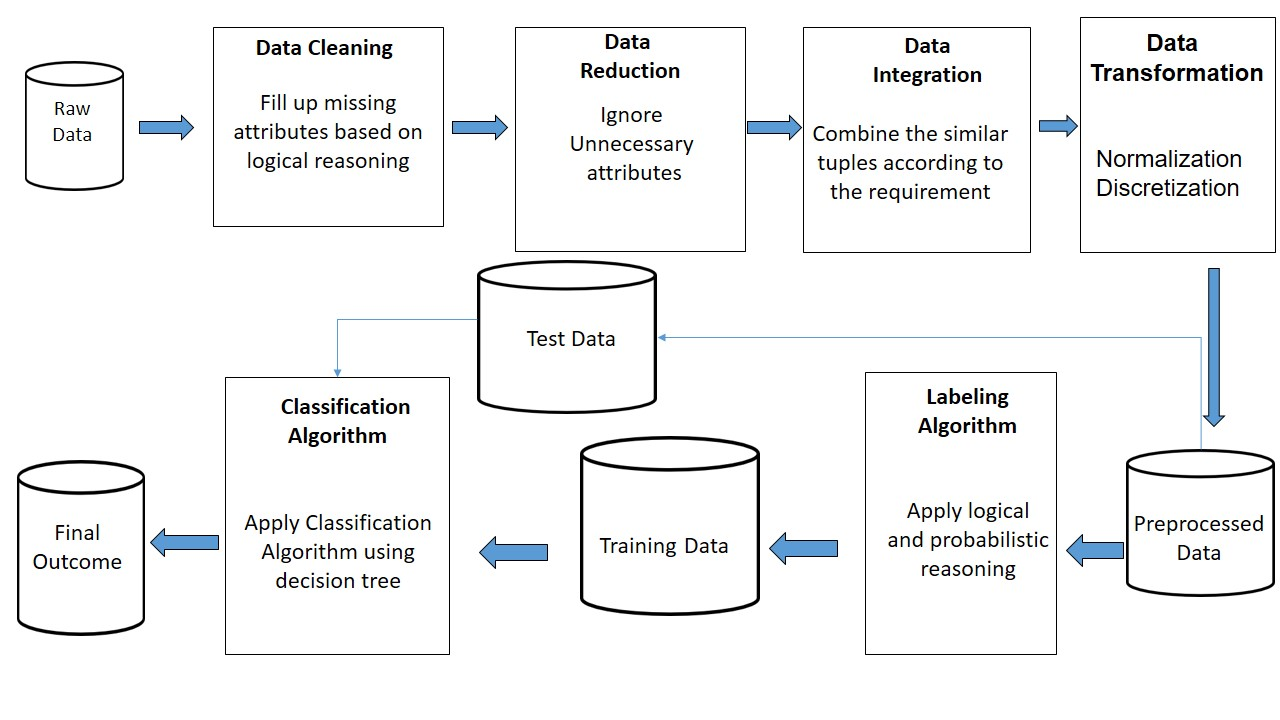
\includegraphics[width=\linewidth]{Figures/classification.jpg}
  \decoRule
  \caption[Classification]{General Process of Classification}
  \label{fig:classification}
\end{figure}

Figure ~\ref{fig:classification} shows the general procedure of classification.
\subsection{Decision Tree Induction}
\paragraph{}
Decision tree induction is the learning of decision trees from class-labeled training tuples. A decision tree is a
flowchart-like tree structure, where each internal node (nonleaf node) denotes a test on an attribute, each
branch represents an outcome of the test, and each leaf node (or terminal node) holds a class label. The
topmost node in a tree is the root node. 
The decision tree in Figure ~\ref{fig:decisiontree} is a tree for the concept buy\_computer that indicates whether a customer at a company is likely to buy a computer or not. Each internal node represents a test on an attribute. Each leaf node represents a class.
The benefits of having a decision tree are 
\begin{itemize}
\item It does not require any domain knowledge.
\item is easy to comprehend.
\item The learning and classification steps of a decision tree are simple and fast.
\end{itemize}
    

\begin{figure}
   \centering
  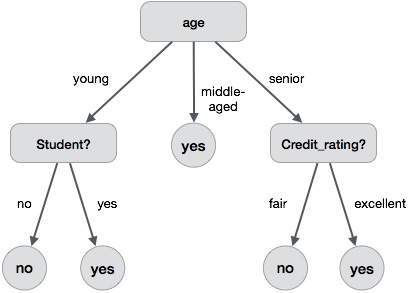
\includegraphics[width=\linewidth]{Figures/dm_decision_tree.jpg}
  \decoRule
  \caption[A Decision Tree]{A Decision Tree}
  \label{fig:decisiontree}
\end{figure}

\subsection{Decision Tree Induction Algorithm}
A machine researcher named J. Ross Quinlan in 1980 developed a decision tree algorithm known as ID3 (Iterative Dichotomiser). Later, he presented C4.5, which was the successor of ID3. ID3 and C4.5 adopt a greedy approach. In this algorithm, there is no backtracking; the trees are constructed in a top-down recursive divide-and-conquer manner.

{\SetAlgoNoLine
\begin{algorithm}[H]

\label{generatedecisiontree}
\SetKwInOut{Input}{Input}
\SetKwInOut{Output}{Output}

\Input{ \begin{itemize}
\item Data partition, D, which is a set of training tuples and their associated class labels;
\item $attribute\_list$, the set of candidate attributes\;
\item $Attribute\_selection\_method $.
\end{itemize}}
\Output{A decision tree.}

\begin{algorithmic}[1]
\caption{Generate\_decision\_tree}
\Procedure{}{}
    \State create a node $N$\;
    \If{tuples in $D$ are all of the same class, $C$,}{
    	return $N$ as leaf node labeled with the class $C$ \;
    }
    
    \If{$attribute\_list$ is empty}{
    	return $N$ as leaf node labeled with the majority class in $D$ \;
    }
   \State apply $Attribute\_selecction\_method(D,attribute\_list)$ to find best splitting\-criterion \;  
        
   \State label node $N$ with $splitting_criterion$ \;
    \If{$splitting\_criterion$ is discrete valued and multiway splits allowed}
   {$ attribute\_list \leftarrow attribute\_list - splitting\_ttribute $\;
   } 
      \For {each outcome $j$ of $splitting\_criterion$}{
        \State let $D_j$ be the set of data tuples in $D$ satisfying outcome $j$ \; 
        \If{$D_j is empty$}
        {
        	attach a leaf labeled with the majority class in $D$ to node $N$ \;
        }
        \Else {attach a leaf labeled with the majority class in $D$ to node $N$ \;}
	}
\State return $N$ \;
\EndProcedure
\end{algorithmic}
\end{algorithm}}

Algorithm ~\ref{generatedecisiontree} is the general approach to build a decision tree.

\subsection{Attributes Selection Measures}
\paragraph{}
An attribute selection measure is a heuristic for selecting the splitting criterion that "best" separates a given
data partition, D, of class-labeled training tuples into individual classes. If we were to split D into smaller
partitions according to the outcomes of the splitting criterion, ideally each partition would be pure (i.e., all the
tuples that fall into a given partition would belong to the same class). Conceptually, the "best" splitting
criterion is the one that most closely results in such a scenario. Attribute selection measures are also known as
splitting rules because they determine how the tuples at a given node are to be split. \newline
The attribute selection measure provides a ranking for each attribute describing the given training tuples. The
attribute having the best score for the measure\footnote{\label{third}Depending on the measure, either the highest or lowest score is chosen as the best (i.e., some measures strive to maximize while others strive to minimize).} is chosen as the splitting attribute for the given tuples. If the
splitting attribute is continuous-valued or if we are restricted to binary trees, then, respectively, either a split
point or a splitting subset must also be determined as part of the splitting criterion. The tree node created for
partition D is labeled with the splitting criterion, branches are grown for each outcome of the criterion, and the
tuples are partitioned accordingly.Three popular attribute selection measures are

\begin{itemize}
\item Information gain
\item Gain ration
\item Gini index
\end{itemize}
The notation used herein is as follows. Let $D$, the data partition, be a training set of class labeled tuples.
Suppose the class label attribute has m distinct values defining m distinct classes, $C_i$ (for $i=1,2,....$). Let
be the set of tuples of class $C_i$ in $D$. Let $|D|$ and $|C_{i,D}|$ denote the number of tuples in $D$ and $C_{i,D}$
respectively.
\subsubsection{Information Gain}\label{infogain}
\paragraph{}
ID3 uses information gain as its attribute selection measure. This measure is based on pioneering work by
Claude Shannon on information theory, which studied the value or "information content" of messages. Let
node N represent or hold the tuples of partition D. The attribute with the highest information gain is chosen as
the splitting attribute for node N. This attribute minimizes the information needed to classify the tuples in the
resulting partitions and reflects the least randomness or "impurity" in these partitions. Such an approach
minimizes the expected number of tests needed to classify a given tuple and guarantees that a simple (but not
necessarily the simplest) tree is found.
\paragraph{}
The expected information needed to classify a tuple in D is given by $$ Info(D)= -\sum(p_i*\log(p_i)) $$
where $p_i$ is the nonzero probability that an arbitrary tuple in $D$ belongs to class $C_i$ and is estimated by $|C_{i,D}|/|D|$. A log function to the base 2 is used, because the information is encoded in bits. $Info(D)$ is just the average amount of information needed to identify the class label of a tuple in $D$. Note that, at this point, the
information we have is based solely on the proportions of tuples of each class. $Info(D)$ is also known as the
entropy of $D$.
How much more information would we still need (after the partitioning) to arrive at an exact classification?
This amount is measured by $$Info_A(D)=\sum{\dfrac{|D_j|}{|D|}*Info(D_j)} $$
nformation gain is defined as the difference between the original information requirement (i.e., based on just
the proportion of classes) and the new requirement (i.e., obtained after partitioning on A). That is,
$$Gain(A)=Info(D)-Info_A(D)$$

\subsubsection{Gain Ratio}
\paragraph{}
The information gain measure is biased toward tests with many outcomes. That is, it prefers to select attributes
having a large number of values. For example, consider an attribute that acts as a unique identifier such as
$product\_ID$. A split on $product\_ID$ would result in a large number of partitions (as many as there are values),
each one containing just one tuple. Because each partition is pure, the information required to classify data set
D based on this partitioning would be $Info_product\_ID(D)=0$ . Therefore, the information gained by partitioning on this attribute is maximal. Clearly, such a partitioning is useless for classification.
\paragraph{}
C4.5, a successor of ID3, uses an extension to information gain known as gain ratio, which attempts to
overcome this bias. It applies a kind of normalization to information gain using a "split information" value
defined analogously with $Info(D)$ as $$SplitInfo_A(D)=-\sum(\dfrac{|D_j|}{|D|}* \log_2(\dfrac{|D_j|}{|D|}))$$
This value represents the potential information generated by splitting the training data set, $D$, into $v$ partitions,
corresponding to the v outcomes of a test on attribute A. Note that, for each outcome, it considers the number of
tuples having that outcome with respect to the total number of tuples in D. It differs from information gain,
which measures the information with respect to classification that is acquired based on the same partitioning.
The gain ratio is defined as $$GainRatio=\dfrac{Gain(A)}{SplitInfo_A(D)} $$

\subsubsection{Gini Index}

The Gini index is used in CART. Using the notation previously described, the Gini index measures the impurity
of D, a data partition or set of training tuples, as $$Gini(D)=1-\sum(p_i^{2}) $$

where pi is the probability that a tuple in $D$ belongs to class $C_i$ and is estimated by $|C_{i,D}|/|D|$ . The sum is computed over $m$ classes.

When considering a binary split, we compute a weighted sum of the impurity of each resulting partition. For
example, if a binary split on A partitions $D$ into $D_1$ and $D_2$, the Gini index of D given that partitioning is
$$Gini_A(D)=\dfrac{|D_1|}{|D|}Gini(D_1) +  \dfrac{|D_2|}{|D|}Gini(D_2).$$

The reduction in impurity that would be incurred by a binary split on a discrete- or continuous-valued attribute
A is $$\delta{}Gini(A)=Gini(D)-Gini_A(D).$$

\subsubsection{Other Attribute Selection Measures}

Many other attribute selection measures have been proposed. CHAID, a decision tree algorithm that is popular
in marketing, uses an attribute selection measure that is based on the statistical $\chi^{2} $ test for independence. Other measures include C-SEP (which performs better than information gain and the Gini index in certain cases) and
G-statistic (an information theoretic measure that is a close approximation to $\chi^{2} $ distribution).\\
Attribute selection measures based on the Minimum Description Length (MDL) principle have the least bias
toward multivalued attributes. MDL-based measures use encoding techniques to define the "best”" decision tree
as the one that requires the fewest number of bits to both (1) encode the tree and (2) encode the exceptions to
the tree(i.e., cases that are not correctly classified by the tree). Its main idea is that the simplest of solutions is preferred. \\
Other attribute selection measures consider multivariate splits (i.e., where the partitioning of tuples is based
on a combination of attributes, rather than on a single attribute). The CART system, for example, can find
multivariate splits based on a linear combination of attributes. Multivariate splits are a form of attribute (or
feature) construction, where new attributes are created based on the existing ones.

